\documentclass[12pt]{report}
\linespread{1.5}
\usepackage{graphicx}
\usepackage{fullpage}
\usepackage{natbib}
\usepackage{float}
\usepackage{subfig}
\usepackage{appendix}

\bibpunct{[}{]}{,}{a}{,}{,}

\begin{document}

\title{Developing a Compiler for the Expert Systems Language, Flex}
\author{05017742 - Thomas Cowell\\
		\texttt{05017742@glam.ac.uk}}

\maketitle

\begin{abstract}
The aim of this project is to create a simple compiler for the expert systems language, Flex.  Flex is an expert systems language that focuses on using plain English to make it accessible for non-technical users, and to aid building rapid rule based systems.
\end{abstract}

\pagestyle{plain}
\pagenumbering{alph}

\tableofcontents

\cleardoublepage
\pagenumbering{arabic}

\chapter{Introduction}
\section{Aim}\label{sec:aim}
The problems outlined in the previous section help highlight the aims and objectives that this project can use.  Time is limited, so it wouldn't be wise to implement a full version of Flex, however a small subset of the language would be sufficient.
\\
\\
This project aims to create a basic compiler of the flex toolkit, using open source software.  The software would be able to be installed on any linux machine, whilst providing the basic features that can run a simple tutorial that help to teach students how to write expert systems.
\clearpage
\section{Objectives}\label{sec:objectives}
The objectives of this project are to:
\begin{itemize}
\item Create a simple flex compiler that can work on the basic tutorials from a tutorial.
	\begin{itemize}
	\item Utilise forward chaining inference engine;
	\item Recognise rules, questions and actions;
	\item Recognise variables, assignments and comparisons;
	\item Work with simple if-statements;
	\item Output variables and text to the user to show results and what's going on.
	\end{itemize}
\item Create it for the Linux platform.
	\begin{itemize}
	\item Command line driven - feed the application a flex source file;
	\item Not be coupled to a Desktop Environment (Gnome, KDE etc);
	\end{itemize}
\item Keep the project open source.
	\begin{itemize}
	\item Keep the project available on a source-control service so it can be ammended to once the project is finished.
	\end{itemize}
\end{itemize}
\clearpage
\section{Abbreviations}\label{sec:abbreviations}
This project focuses on two technologies called Flex.  The project focuses on the expert systems language 'flex', which is a toolkit as part of WinProlog.  The other flex is the 'Fast Lexical Analyser', which takes an input source file and generates tokens from regular expressions.  To avoid confusion, the expert systems language Flex will be called 'WinFlex' from now on, because of its assosciation with Win-Prolog.
\section{Project Contents}\label{sec:project_contents}
The following sections will discuss the overall layout of how this paper will look.
\subsection{Chapter 2: Literature Review}\label{sec:sub:chapter2}
The literature review shall introduce the motiviation behind the choice of the title for this project.  This will cover the problems of the current software solution to help educate students about expert systems and WinFlex.  Artificial intelligence, expert systems, Prolog and WinProlog will also be discussed.  The literature review will also look to see if there has been any similar research, and if there is, discuss how the author went about researching and implementing their solution.
\subsection{Chapter 3: Research}\label{sec:sub:chapter3}
The research chapter will introduce Artificial Inteligence, expert systems and the various stages that make up a compiler.  The research shall also be looking into Linux as a development environment, including the  flex and bison packages, plus the GCC compiler.  Finally, a small section will discuss source control, which allows the code to be stored centrally, providing useful tools such as revision control, back up, multi-develoer collabortion and more.
\subsection{Chapter 4: Implementation}\label{sec:sub:chapter4}
The implementation chapter will discuss the design process of the compiler.  This shall cover details such as what features should be built into the compiler, based on research into WinFlex tutorials that were worked on in some modules.  This will involve creating the tokens for the parser, and thus, designing the grammar around the current WinFlex implementation as close as possible.  Finally, data structures will be discussed, more specifically, Abstract Syntax Trees, as they provide the backbone to storing data before turning the code into something meaningful for the machine to understand.
\subsection{Chapter 5: Testing}\label{sec:chapter5}
The testing chapter will provide an overview of the tests carried out.  The actual test files will be found in the appendix, but the expected results, description and actual result will be found here.  For any tests that fail, there will be a discussion of why it failed and how the problem can be fixed.
\subsection{Chapter 6: Conclusion}\label{sec:sub:chapter6}
The conclusion will discuss what was achieved and learnt.  It shall discuss whether the end product met the aims and objectives set out in the introduction and if anything went wrong, then it shall ask why it went wrong and what could have been done to prevent it if there were an opportunity to repeat the task.  Finally, the conclusion will discuss any work that could be carried out in future, or if there weren't the same time restranints.
\chapter{Literature Review}
\section{Project Motivation}\label{sec:project_motivation}
Before this paper begins, it is worth noting the motivation behind this project.  Certain modules on the 'Intelligent Computer Systems' course required the use of a propietary software package called WinProlog.  The application can do a wealth of tasks, however, the modules only focused on a niche feature of the software, a toolkit based on Prolog called Flex (abbreviated to WinFlex to avoid confusion with the Lexixcal Analyzer, Flex).  WinFlex allows professionals, engineers and students alike to quickly write a rule-based system using a language that is very close to the English language.
\\*
\\*
Whilst WinFlex achieved results, it was felt that the debugging features were sub-par and were often inaccurate, giving no helpful messages for a beginner to use to correct their mistakes.  Also, because of the restrictions of having a licence, it meant that the software could only be installed on certain machines, in a different department within the University campus, which students felt was restrictive and inconvienient.
\\
\\
\\
\\
\begin{figure}[h!]
	\centering
		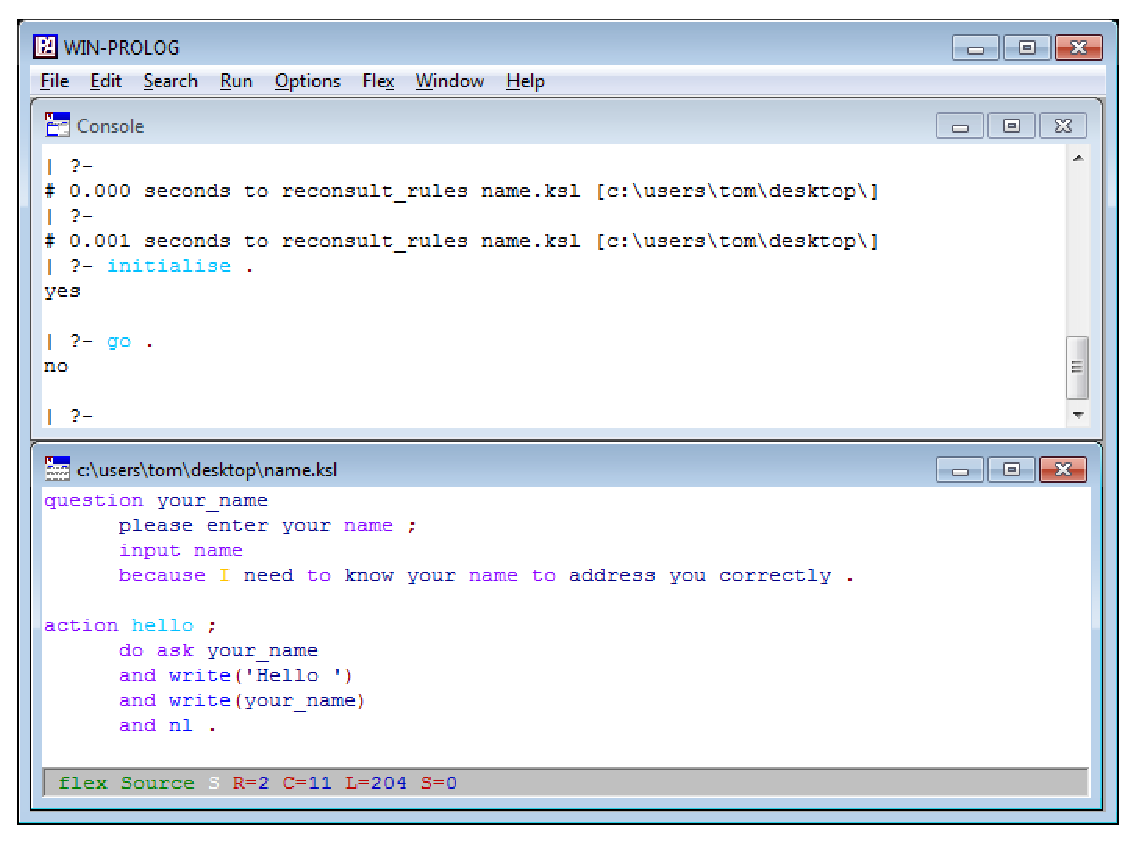
\includegraphics[scale=0.85]{flexfail}
		\caption{A simple flex program that is syntatically wrong, plus the resulting error.}\label{fig:flexfail}
\end{figure}
\\
In figure \ref{fig:flexfail}, the line \texttt{input name} should have a semi-colon at the end, like 
\begin{center}
\texttt{input name ;}\\
\end{center}
to let the compiler know that the line is finished, but the question isn't over.  Whilst this is a simple mistake, the WinFlex compiler hasn't picked it up, and is only being discovered when trying to run the action \texttt{go}, where WinFlex returns an error message \texttt{no}, with no indiciation what the error is, where it is or how to fix it.  If this were a large set of rules, finding such a basic mistake could take a long time to fix.\\
\\
The figures \ref{fig:flex_error1} and \ref{fig:flex_error2} show flex encountering a gramatically incorrect script, with the compiler displaying errors.
\begin{figure}[H]
	\centering
		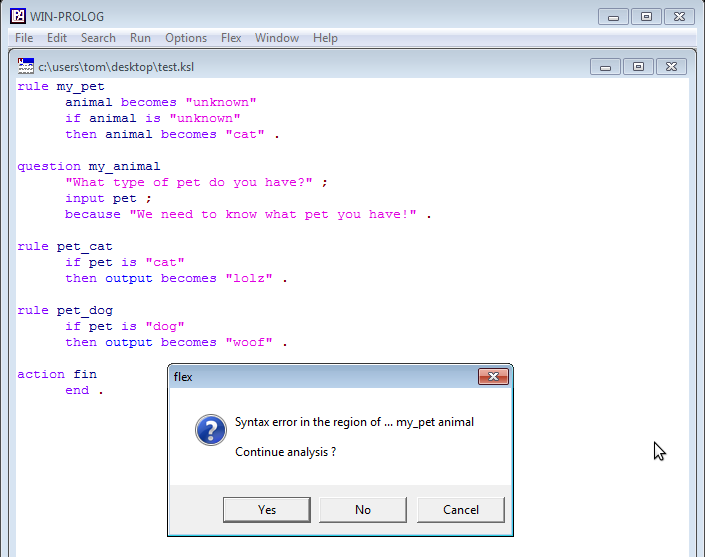
\includegraphics[scale=0.65]{flex_error1}
		\caption{The compiler has detected an error in the grammar.}\label{fig:flex_error1}
\end{figure}
Whilst the compiler in WinProlog does try to track down the error, it's not very friendly to new users, as it doesn't let them know where the error is, or what is wrong.  There were situations where n tutorials and in courseworks, where by small, simple errors could have been easily fixed if it weren't for ambiguous language on the debugger.
\begin{figure}[H]
	\centering
		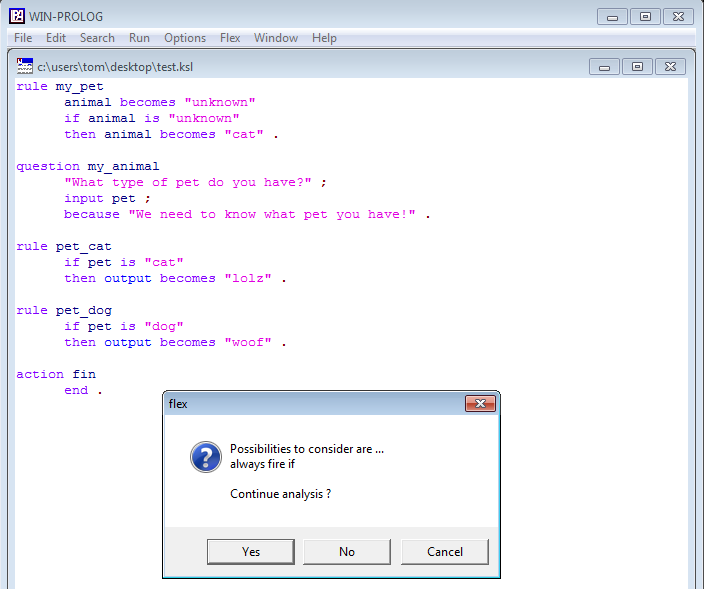
\includegraphics[scale=0.65]{flex_error2}
		\caption{The compiler error isn't very specific to where it is refering to, there are no line number or highlighting on the error.}\label{fig:flex_error2}
\end{figure}
Figure \ref{fig:flex_error2} shows an error message for the example code.  Even though most of the code is gramatically wrong, the compiler insists that the error is at the top, where the first rule is gramatically sound.
\clearpage
\section{Outline}\label{sec:outline}
As described in chapter 1, the outline of this project is to create a compiler for the expert systems language, WinFlex.  Whilst WinFlex is based on the Artificial Intelligence langauge Prolog, this basic compiler will be written in C, emulating the basic features of WinFlex, mainly as a teaching tool, rather than a fully fledged toolkit.

\section{Previous Work}\label{sec:previous_work}
Because the WinFlex toolkit is unique, there aren't many examples or previous work done on creating a compiler primarily for the langauge.  However, there are countless items of literature dedicated to writing compilers, all for different languages, but constructed in the same manor - using flex, bison and gcc.

\subsection{Paper 1}\label{subsec:paper1}
\textbf{Paper:} Compiler Design for Efficient Code Generation and Program Optimization\\
\textbf{Author:} A. Rudmik and E.S. Lee\\
\textbf{Year:} 1979\\
\\
The first paper to be looked at discusses an approach to designing a compiler for Pascal language.  Whilst it isn't the same language as WinFlex, it should have the same principles regarding compiler construction.  The paper has it's draw backs though, as it was written in 1979, the chances that compiler construction and design have changed is quite likely, or at least certain techniques may have changed.\\
\\
The paper discusses "passes" of the compiler, different stages that the compiler goes through in order to take the source code and turn it into a native program.  The following quote from the paper looks briefly into the several passes that the Pascal compiler goes through to take the source program and turn it into a native machine runable application.
\paragraph{Pass1} performs the lexical and syntactical analysis, generating as output a standardized high level control flow graph.
\paragraph{Pass2} analyzes the constant, type, and variable declarations and maps the program identifiers into unique name indicies according to PASCAL scope rules.
\paragraph{Pass3} traverses the control flow graph and checks the program for semantic correctness.  In the process of performing the semantic analysis, simple transformations are performed on the flow graph in instances where the graph generated in pass1 does not represent teh semantics of the program.
\paragraph{Pass4} replaces the calls to open procedures by the corresponding procedure bodies.  Temporary storage locations are assigned to local variables declared within open procedures.
\paragraph{Pass5} performs global machine and lanaguage independent optimizing transformations on the intermediate code.
\paragraph{Pass6} performs a "live-dead" variable analysis and encodes this information in the flow graph to be used by the register allocator in pass7.
\paragraph{Pass7} translates the intermediate code into machine specific object code.
\paragraph{Pass8} performs machine dependent peephole optimizing transformations on the object code. \citep{compilercodegeneration79}\\
\\
Passes 1 to 4 represent the stages of lexical analysis, parsing the grammar, building the syntax up into a syntax tree and then checking the data types on expressions, making alterations to some data types where deemed necessary, and finally, generating the intermediate code.
\\
Passes 5 to 8 discusses the phases of the compiler that optimise the intermediate code and turns it object code, which in turn is optimised further into machine code for the specific platform.\\
\\
The paper continues to go into greater depth about the specifics of a Pascal compiler.
\chapter{Research}
\section[Research]{Research}\label{sec:intro_to_research}
Before any implementation can begin, research needs to be conducted in order to gain a better understanding about expert systems, the WinFlex language and various toolkits for developing compilers.

\section{Artificial Intelligence}\label{sec:AI}
Artificial Intelligence (AI) is a term for machines that can appear to act as if they are 'thinking' for themselves - that is, to emulate the way the human mind works.\\
\\
Roughly speaking, Artificial Intelligence is the study of man-made computational devices and systems which can be made to act in a manner which we would be inclined to call intelligent. \citep{whatisai}
\\
\\
Interest in AI began when the British computer scientist Alan Turing stated, that if a machine can pass a series of questions, and trick the questioner into thinking that the machine was infact human, then the machine could be classed as having intelligence.  This test has since become known as the 'Turing Test', and is still used today as an acid test to test the capability of an AI implementation.\\
\\
Artificial Intelligence can be applied to many areas, such as computer controled characters in computer games (NPC's), banking systems to detect fraudulant transations (neural networks can 'learn' the habbits and behaviours of customers, anything that breaks the pattern is detected, and the customer is notified), and systems that aid professionals to reach decisions that otherwise may take a lot of consideration.
\\
\\
Expert Systems fall into the category of AI, because they emulate the roll of an expert of a field.  Given answers, an expert system should be able to come to a conclusion based in varying pieces of information.
\section{Expert Systems}\label{sec:expert_systems}
In the modern world where information is highly valuable and where time is of the essence, many experts have turned to computing to help provide answers for them that may otherwise take a while to reach through their own expertees, or where a human expert may forget all the approaches into a decision making process.  Expert Systems provide an easier way for professionals to reach conclusions through a series of questions, usually linking to a knowledge base.  For example, a doctor may use an expert system to reach a diagnosis for a patient where the illness or problem may not be readily obvious.  The system would ask a question where the doctor would answer with the symptoms, and then the expert system would continue asking more questions, based on the previous answers, until a conclusion is reached.
\\*
\\*
Expert system development entials the conversion of information about a bounded problem domain into knowledge, which is then represented in a format suitable for computer manipulation.  The created depository of knowledge, known as the knowledge base, can then by used by various deductive reasoning techniques to derive solutions \citep{expertsystems98}.
\\*
\\*
From this, it is obvious that the usefulness of the expert system is only as good as the underlying data - the knowledge base.  Using the doctors example from the previous paragraph, the system would be of no use if the knowledge base had minimal content, whilst in the reverse situation, it would be extremely useful to have a large knowledge base.  Doctors from around the world could contribute answers as new illnesses and cures are discovered, which in turn would improve the accuracy and usefulness of the expert system.
\\*
\\*
At the heart of an expert system is an inference engine.  The engine attempts to pick out an answer from a knowledge base
\\*
\\*
Expert systems can be found in many areas of industry, including engineering, medical, financial forecasting, or even just personal information systems for helping customers at a shopping centre.
\\*
\\*
Expert systems languages are entirely different to imperative languages such as C, C\#, Java.  Instead, they make use of logical langauges, such as Prolog, which is based on rules, and assosciations with data.  The code in figure \ref{fig:prolog_code} shows a short example of a program written in Prolog.
\\*
\\*
\begin{figure}[H]
\texttt{born(charles, elizabeth2, philip).\\
born(anne,    elizabeth2, philip).\\
born(andrew,  elizabeth2, philip).\\
born(edward,  elizabeth2, philip).\\
\\
born(diana,   frances,    edwardSpencer).\\
\\
born(william, diana,      charles).\\
born(henry,   diana,      charles).\\
\\
? born(S, elizabeth2, Y) and born(G, M, S).}
\caption{Example Prolog code.\citep{thehouseofwindsor}}
\label{fig:prolog_code}
\end{figure}
The first four lines link the first argument with the next two.  So, on line one, charles is the child of elizabeth2 and philip.  On the 5th line, diana is declared as the daughter of frances and edwardSpencer.  The final line executes the program, by submitting a query.
\\*
\begin{figure}[H]
\texttt{born(charles, elizabeth2, philip), born(william, diana, charles) yes\\
born(charles, elizabeth2, philip), born(henry, diana, charles) yes}
\caption{Output from executing the sample code.}
\label{fig:prolog_output}
\end{figure}
Figure \ref{fig:prolog_output} shows the output from the sample code.  The query executes two sub queries, \texttt{born(S, elizabeth2, Y)}, which retrives a set of data where the child's mother is \texttt{elizabeth2}.  Based on the four rules at the start of the program, this would return four answers for \texttt{S}, and a single result for \texttt{Y} (philip).  The second query, \texttt{born(G, M, S)} queries the returned data set from the first query.  In this case, the mother (\texttt{M}), while the father is \texttt{S}.  Lines six and severn in figure \ref{fig:prolog_code} show that charles has two children, and thus \texttt{william} and \texttt{henry} are returned.
\clearpage
\subsection{Disadvantages}\label{subsec:disadvantages_expert_systems}
There are some notable disadvantages to expert systems.  An important pitfall to consider is the GIGO acronym - Garbage In Garbage Out.  If the rules aren't built properly, or if the person using the system enters incorrect data, then the system will produce an incorrect answer, but the user may take it for granted that the system is always correct.  Also, if the person being questioned gives an answer that they're uncertain of, then the result may not be accurate, and the expert system would be non-the wiser.  A human expert would be able to tell the certainty of someones answer, and possibly re-ask the question in a way that the questionee would understand.

\section{WinProlog}\label{sec:winprolog}
WinProlog is a propietary software package, developed by Logic Programming Associates Ltd.  LPA describe Win-Prolog below:
\\*
\\*
WIN-PROLOG is the leading Prolog compiler system for Windows-based PCs. Prolog is an established and powerful AI language which provides a high-level and productive environment based on logical inference.\citep{lpawinprolog}
\\*
\\*
One of the features of Win-Prolog is Flex, an expert systems toolkit built on top of Prolog.

\section{Flex (WinFlex)}\label{sec:introflex}
The 'WinFlex Tutorial' describes WinFlex as "Flex is a software system specifically designed to aid the development and delivery of Expert Systems."
\\*
\\*
To appreciate both the power and limitations of Expert System approaches to reaching expert conclusions, it is necessary to construct and experiment with expert systems.  In this module, the Flex Expert System Shell will be used.  Flex describes knowledge in terms of \textit{production rules} (that is, \textit{if-then} statements), which has proved the most popular approach to encapsulation expert knowledge.  Such rules, despite appearing simple, enable relatively complex connections to be made between individual pieces of 'knowledge', thereby solving apparently difficult problems.\citep{flexsystems09}.
\\*
\\*
The advantages of WinFlex is that it's easy to understand, as it's very close to the English language.  A non-programmer could look at it and understand the system within several minutes, where as a traditional Prolog script may need some prior understanding of programming to be able to understand what is going on.
\\*
\\*
Flex expert system toolkit, an expressive and flexible rule-based development system for building and delivering scalable and flexible expert systems and business rules applications. Flex provides a comprehensive and versatile set of facilities for both programmers and non-programmers to construct reliable and maintainable applications.\citep{lpawinprolog-flex}.
\\*
\\*
WinFlex is capable of working with the knowledge base in two distinct ways: Forward and Backward chaining.  The differences are described below.
\subsection{Forward Chaining}\label{subsec:forward_chaining}
Forward chaining is a method of reasoning in expert systems.  In laymens terms, forward chaining looks at what the system knows, and asks questions to get more information in order to reach a conclusion by using if-then statements to determine the value of objects, through a series of rules.
\clearpage
If a rule relies on knowing the value of an object (\textit{i.e.} because it is used in a condition), one of the following three cases applies:
\begin{itemize}
	\item the object has already been instantiated;
	\item the object has not yet been instantiated, but the inference engine can find a question to ask which will determine its value - this causes WinFlex to ask the question;
	\item the object has not yet been instantiated, but the inference engine can find another rule which might determine its value. \citep{forwardchaning09}
\end{itemize}
Basically, the flow of the program is determined by whether or not objects are instantiated (created and have a value) or not.  The inference engine will try its best to obtain a value, from either another rule or by asking a question.\\
\\
An example of this usage, would be where an expert system asks a user for a series of symptoms in order to try and work out the illness.
\subsection{Backward Chaining}\label{subsec:backward_chaining}
As the name suggests, backward chaining is the opposite of forward chaining.  Backwards chaining works from a goal, and attempts to see if there is any data to support its goal.  If not, it moves into the next goal, and tries again.  Rather than using rules, backward-chaining programs use 'relations'.  The easiest way to explain is by using an example.\\
\begin{tabbing}
	\texttt{relation} \= \texttt{determine\_mood(irritable)}\\
	\> \texttt{if day is 'Monday'}\\
	\> \texttt{and time is 'early'} .\\
\end{tabbing}
The relation above would become 'irritable' as long as both tests are true - day must be 'Monday' and time is 'early'.  There can be multiple relations of the same name, in this case, 'determine\_mood' with different objects (irritable), so, the above relation could co-exist along with the relation below, where each relation would fire in the order they appear in the program:
\begin{tabbing}
	\texttt{relation} \= \texttt{determine\_mood(happy)}\\
	\> \texttt{if day is 'Friday'}\\
	\> \texttt{and time is 'afternoon'} .\\
	\\
	\texttt{action} \= \texttt{go}\\
	\> \texttt{do restart}\\
	\> \texttt{and determine\_mood(Mood)}\\
	\> \texttt{and report(Mood) .}\\
\end{tabbing}
The above program would fire both relations, and the value of Mood would become either irritable or happy, depending if the tests are true.
\clearpage
\subsection{Forward Chaining Examples}
The code below shows an example program written in WinFlex, using forward chaining:
\begin{figure}[H]
	\begin{tabbing}
		\texttt{group} \= \texttt{temperature\_choices warm, cold .}\\
		\\
		\texttt{rule ask\_temperature} \\
		\>	\texttt{if the temperature is unknown}\\
		\>	\texttt{then ask temperature .}\\
		\\
		\texttt{question temperature}\\
		\>	\texttt{What is the temperature?;}\\
		\>	\texttt{choose from the temperature\_choices ;}\\
		\> 	\texttt{because it is necessary to work out the need for a coat .}\\
		\\
		\texttt{rule} \= \texttt{temp\_w}\\
		\>	\texttt{if temperature is warm}\\
		\>	\texttt{then write('You would be mad to wear a coat.').}\\
		\\
		\texttt{rule} \= \texttt{temp\_c}\\
		\>	\texttt{if temperature is cold}\\
		\>	\texttt{then write('Take a coat to keep warm.').}\\
		\end{tabbing}
		\end{figure}
		% break up the float so it can span two pages.
		\begin{figure}[H]
		\begin{tabbing}
		\ContinuedFloat
		\texttt{ruleset} \= \texttt{take\_a\_coat}\\
		\>	\texttt{contains all rules;}\\
		\>	\texttt{select rule suing first come first servced;}\\
		\>	\texttt{update ruleset by removing each selected rule;}\\
		\>	\texttt{initiate by doing restart .}\\
		\\
		\texttt{action} \= \texttt{go}\\
		\>	\texttt{do invoke ruleset take\_a\_coat .}\\
	\end{tabbing}
	\caption{A simple flex program that lets you know if you should wear a coat or not.}
	\label{fig:flex_code}
	\citep{flexsystems09}
\end{figure}
It's immediately obvious that the program is made up of rules and questions.  The compiler starts from the top, and runs down through the rules, until they've all been fired.  Questions only get fired if they are called upon within a rule.\\*
\\
The first line declares a group of choices that can be asked during a question.  This can be likened to a Enumerative type in languages such as C and C\#, where \texttt{warm} and \texttt{cold} are two options that belong to \texttt{temperature}.  The first rule, \texttt{ask\_temperature}, checks if the variable \texttt{temperature} (not to be confused with the group of the same name) has been assigned a value.  If it's not, then it asks the question, \texttt{temperature}.  Because the WinFlex compiler starts at the top, then temperature will be unknown by default, so this rule will always fire.\\
\\
Questions always have the same format: The first line is the question text that the user will see, the second line presents the options to the user and also accepts their input.  In this instance, the user will be presented the two choices of \texttt{temperature}, where the choice is then assigned to the variable \texttt{temperature}.\\
\\
The two rules, \texttt{temp\_w} and \texttt{temp\_c}, check the users input, and display the message as appropriate, while the ruleset \texttt{take\_a\_coat} tells the compiler how to go about running the script.  Finally, the the action \texttt{go}, which is triggered as a query from the command prompt, starts the program.\\
\\
Whilst this is a reasonably simple script, it has all the basics that make up larger and more complicated flex programs.

\section{What Is A Compiler?}\label{sec:what_is_a_compiler}
In laymens terms, a compiler takes human readable source code and translates it into a language that the machine can understand.\\
\\
Programming languages are notations for describing computations to people and to machines.  The world as we know it depends on programming langauges, because all the software running on all the computers was written in some programming langauge.  But, before a program can be run, it first must be translated into a form in which it can be executed by a computer.

The software systems that do this translation are called \textit{compilers}.\citep{compilers07}
\\*
\\*
This quote gives a brief overview of what a compiler does.  It translates the human readable program into a format that the computer can understand, i.e. instructions.  Whilst this sounds simple, the actual process is reasonably complicated, and done in several phases:\\
\begin{itemize}
	\item Lexical Analysis
	\item Syntactical Analysis
	\item Intermediate Code Generation
	\item Optimization
	\item Object Code Generation
\end{itemize}\citep{compilerconstruction92}
\subsection{Lexical Analysis}\label{subsec:lexical_analysis}
The first task of the compiler is to read the source code that the developer has written, and breaks it up into meaningful chunks called tokens.  These tokens are defined in a lexical file, in which the lexical scanner will process.  For example, take the following flex code:\\
\texttt{\begin{tabbing}rule \= my\_pet\\
\>	if animal is 'cat'\\
\>	then sound becomes 'meow' .\\
\end{tabbing}}
The code is made up of several different types of 'words'.  Some are specific to the language (keywords), some identify a variable (identifiers) whilst others perform a certain operations (operators).  This can be broken down to be easier to understand:\\*
\begin{itemize}
	\item keywords: rule, if, is, then
	\item identifiers: my\_pet, animal, sound
	\item operator: becomes
	\item string: 'cat', 'meow'
	\item punctuation: .\\
\end{itemize}
The lexical analyser is capable of removing characters that aren't relevant to the program, such as comments, new lines and whitespace (spaces and tabs).  All of the above are leximes that are mapped into tokens, that makes it easier for the syntactic analyser to understand.  The way that the lexical analyser recognises these leximes is through matching the patterns of text, which is where regular expressions come in useful.\\
\subsubsection{Regular Expressions}\label{subsubsec:regex}
Regular Expressions, often identified or shortned to 'regex', allows developers to match patterns of text.  It is extremely powerful for recognising patterns in text, and seeing as a programming language is made up patterns, is used in the lexical analysis process for matching expressions to create tokens.
\\*
\\*
A regular expression is a pattern description using a metalanguage, a language that you can use to describe what you want the pattern to match.  Flex's regular expression language is essentially POSIX-extended regular expressions (which is not surprising considering their shared Unix heritage). \citep{flexandbison09}
\\*
\\*
Regular expressions are a powerful way of matching complicated patterns of strings.  It uses a series of special characters that allow the user [of regular expressions] to create a query.
\\*
For example, numbers can be expressed in several ways, some numbers are negative and some have decimal places.  An expression needs to be able to recognise these different formats.  A string of digits, which can either be positive or negative, can be represented using the expression below:\\*
\\*
\texttt{[-+]?[0-9]+}
\\*
\\*
The square brackets \texttt{[ ]} represents a character class, matching anything within the brakcets.  The first occurance, \texttt{[-+]} matches either a postive of a negative symbol at the start of the expression.  The \texttt{?} character means that the preceding character class can either occur once, or never, which means that the plus or minus characters can be optional.  Next is the \texttt{[0-9]} expression, which matches any text that is number 0 to 9 - the \texttt{+} at the end means that the preceeding expression can be matched one or more times, allowing a number to be either 1 or 12345.  Another example, shown below, recognises an identifier, such as one from the flex example.
\\*
\\*
\texttt{[a-zA-Z\_][a-zA-Z0-9\_]*}
\\*
\\*
The expression is comprised of two character classes.  The first matches a series of characters, in either lower or uppercase, followed by an underscore. The following class is similar, but can also contain numbers.  The astricks, \texttt{*}, means that the preceeding expression can be matched zero or more times, so, the second character class is optional.  This example allows for an identifier to look something like:\\
\\
\texttt{animal}\\
\texttt{My\_Animal01}\\
\texttt{animal\_}\\
\\
But \textbf{not}:\\
\texttt{my1\_animal}\\
\texttt{1\_animal}\\
\\
Matching keywords is much easier, as they need to be treated literally.  Matching for the \texttt{if} keyword, for example, simply looks like so:\\*\\*
\texttt{"if"}
\subsection{Syntactic Analysis}\label{subsec:syntactical_analysis}
The process of syntactic analysis is to parse the tokens into meaningful sentences.  It creates a tree of tokens, whereby each node represents an operation such as \texttt{while}, and its child nodes represent the evaluation expression, and the block of code to loop around, which could be broken down again, where the evaluation is the root node, and the children are the parameters and comparison operators.
\begin{center}
\texttt{\begin{tabbing}while \= (found != true) \{\\ \> found = do\_something();\\ \}\end{tabbing}}
\end{center}
The code above can be broken down into tokens.
\begin{itemize}
	\item Keywords: while, true
	\item Identifiers: found, do\_something
	\item Operators: =
	\item Comparison: !=
	\item Punctuation: \{ \} ( ) ;
\end{itemize}
\begin{figure}[H]
	\centering
		\includegraphics[scale=1]{whilegraph.ps}
		\caption {Expression parse tree.}\label{fig:whilegraph}
\end{figure}
Figure \ref{fig:whilegraph} shows a parse tree of the simple \texttt{while} code sample.  The code is broken down into two main parts - the evaluation, and the block.  These are then further broken down further down the tree.\\
\\
The syntactic analyzer, or \textit{parser}, is the heart of the front end of the compiler.  The parser's main task is analyzing the structure of the program and its component statements and checking these for errors.  It frequently controls the lexical analyzer, which provides tokens in response to the parser's requests, and it may also supervise the operation of the intermediate code generator.\citep{compilerconstruction92}
\\*
\\*
A programming langauge follows a strict set of rules that form it, much like the English langauge has rules to string certain words together to form meaningful and sensible sentences.  The parsers job is to put the tokens into an order that follows the grammar, and put the tokens into a syntax tree, following the rules of the grammar.  For example, the grammar specifies that an identifier, or an expression, must come after the \texttt{if} keyword, followed by a comparison of another identifier or expression.
\subsubsection{Grammar}\label{subsubsec:grammar}
For the parser to operate, there needs to be a way for the syntactic analyser to convert the tokens into the parser tree.  The grammar fulfills this role by using a BNF, or EBNF.  It originally started as BNF (Backus-Naur Form), as created by John Backus and Peter Naur to describe the syntax of a specific language.\\*
\\*
John Backus and Peter Naur introduced for the first time a formal notation to describe the syntax of a given langauge (This was for the description of the ALGOL 60 programming langauge. \citep{whatisbnfnotation}
\\*
\\*
The grammar is the important area of the parser, as it defines how the langauge should look and work.  Most langauges use "context free grammars", where the grammar is built up of small chunks, which can be used in themselves in a recursive fashion.\\*
\\*
Context-free grammars are used to describe the syntactic structure of programs of a programming language.  This shows how programs are composed from subprograms, or, more precisely, which elementary constructs there are and how composite constructs can be built from other constructs. \citep{compilerdesign95}\\*
\\*
Take the following EBNF grammar for example:\\*
\begin{figure}[H]
\begin{tabbing}
\texttt{stmt:}\= \texttt{ if\_stmt}\\
\>\textbar \texttt { while\_stmt}\\
\>\texttt{;}\\
\\
\texttt{if\_stmt:}\= \texttt{ IF test THEN expr ELSE expr}\\
\>\textbar \texttt{ IF test THEN expr}\\
\>\texttt{;}\\
\\
\texttt{while\_stmt:}\= \texttt{ WHILE '(' test ')' '\{' expr '\}'}\\
\>\texttt{;}\\
\end{tabbing}
\caption{Conext Free Grammar in EBNF}\label{fig:context_free}
\end{figure}
Figure \ref{fig:context_free} shows three rules, \texttt{stmt}, \texttt{if\_stmt} and \texttt{while\_stmt}.  The root rule here, \texttt{stmt}, contains two further rules, which can either be an if statement, or a while statement.  These statements are then declared seperately below, where \texttt{if\_stmt} declares two types of if statements that are allowed.  The if statement can either consist of an if-then-else, or an if-then statement.  These rules also contain other rules nested inside of them, such as \texttt{test} and \texttt{expr}, however they aren't listed for the purpose of the example.  The keywords are clearly visible, as they are represented in capital letters.
\subsubsection{Parsing}\label{subsec:parsing}
Parsing is the process of constructing the syntax tree from the grammar.  There are two different ways of performing this task, both of which are described below.
\paragraph{Top-Down Parsing}
The top-down parser begins with the start symbol in the grammar, and with the use of the token stream, tries to predict which is the next route to take to get to the end result.\\
\\
The top-down parser must start at the root of the tree and determine, from the token stream, how to grow the parse tree that results in the observed tokens.  It must do this from nothing but knowledge of the incoming tokens and of the productions in the grammar.  Furthermore, as a practical matter, it must scan the incoming tokens from left to right. \citep{compilerconstruction92}
\\
This quote gives a basic overview of how the top-down parsing process works.
\paragraph{Bottom-Up Parsing}
A bottom-up parser attempts to perform the parsing the opposite way of top-down, in that it starts at the leaf nodes, and works its way to the root.  Bottom-up parsing is much more powerful, but more complex, than top-down parsing.
\subsection{Syntax Trees}\label{subsec:syntax_trees}
Data structures are programming constructs that allow the storage of related data.  They are advantageous as they are quick to traverse and easier to manage than a flat storage system.  For the context of a compiler, they are useful for storing the logic of the code in a tree.  This is where syntax trees are useful.\\*
\\*
One of the most powerful data structures used in compilers is an \textit{abstract syntax tree} (AST). ... In most real grammars, there are rules that exist to manage grouping but that add no meaning to the program.  An AST is basically a parse tree that omits the nodes for the uninteresting rules. \citep{flexandbison09}\\
\\
So while syntax trees are similar to parse trees, they differ in that syntax trees only store the programming constructs, whilst the parse tree represents rules in the grammar that may simply group other rules together, thus creating a smaller, lighter data structure.\\
\\

\subsection{Semantic Analysis}\label{subsec:syntax_trees}
The semantic analyser checks the syntax tree and symbol table for consistency against the source program.\\
\\
The \textit{semantic analyser} uses the syntax tree and the information in the symbol table to check the source program for semantic consistency with the langauge definition.  It also gathers type information and saves it in either the syntax tree or the symbol table, for subsequent use during intermediate-code generation. \citep{compilers07}\\
\\
The semantic analyser also has the job of checking data types in expressions.  For example, it will check that in a statement:
\begin{center}
	\texttt{a = b * c}\\
\end{center}
has the correct data types, where \texttt{b} and \texttt{c} shoud be numerical types, and not a string or boolean.  The semantic analyser can also detect similiar types that can be used together for certain operations, such as using floating point numbers and integers.  If an expression contains a mixture of floating point numbers and integers, the compiler may 'convert' the integer into a float to make the number compatible.
\subsection{Intermediate Code Generation}\label{subsec:intermediate_code_gen}
Intermediate Code Generation is the next stage of the process.  The basic gist of it is that it transforms the parse tree generated by the parser into an intermediate language representation.  The intermediate langauge means that it can run on any machine architecture, i.e., it's not specific to an AMD64 processor instruction set.  The langauge is unoptimised, however, so the later stages of the compiler are important to optimise and convert to the machines native langauge.  The intermediate language can be found for common languages such as Java (Java Virtual Machine) or for .NET.  Prolog has a specific intermediate language called the 'Warren Abstract Machine'.\\
\\
There are two types of intermediate code generators:
\paragraph{High-Level Representations} are closer to the source langauge, i.e. the langauge that is being compiled.  They are generally easy to compile, however they are more difficult to optimise.  Syntax trees are an example of a high-level representation of intermediate code.
\paragraph{Low-Level Representations} are closer to machine language, and are usually easier to optimise, as the target architecture is known.  This could be useful where speed and efficiency is critical.
\subsubsection{Warren Abstract Machine}\label{subsubsec:wam}
The Warren Abstract Machine (WAM) is a compiler specifically for Prolog.
\subsubsection{LLVM}\label{subsubsec:llvm}
LLVM (Low-Level Virtual Machine) is a framework that helps to create the intermediate code for a compiler.  It is unrelated to the actual Virtual Machines that run full desktops on top of another desktop.  One of the main sub-projects of LLVM is:\\
\\
The LLVM Core libraries provide a modern source- and target-independent optimizer, along with code generation support for many popular CPUs (as well as some less common ones!) These libraries are built around a well specified code representation known as the LLVM intermediate representation ("LLVM IR"). The LLVM Core libraries are well documented, and it is particularly easy to invent your own language (or port an existing compiler) to use LLVM as a optimizer and code generator. \citep{llvm10}
\\
\\
In short, LLVM can provide a way of optimizing and generating the object code for a wide range of processor archiectures.  Whilst LLVM is specifically designed for C++, there is a project, called Clang, that provides a C based (C, C++, Objective-C) front end (the lexical analysis and parsing phase), making it even easier to generate the AST's and feed it into LLVM.
\subsection{Optimization}\label{subsec:optimization}
The intermediate code generation stage produces a lot of code that is over-complicated, which can in turn slow down the speed of the compiled code.  The optimisation process removes the uncessary code and helps to make the object code more efficient.  Not all compilers contain an optimisation processes - some compilers with the intent to teach programming may not have an optimisation module built in, as it doesn't fit the requirements of the user.  However, for more practical situations, the optimiser is essential, and could make a significant difference when compiling a large project.\\
\\
A compiler for use in teaching programming does not need to produce efficient code.  This is because the bulk of a student's time will be spent in debugging; the program will normally be re-compiled every time it is run.  Once the program is to all appearances correct, the student will hand it in and never run it again. \citep{compilerconstruction92}\\
\\
The advantage of optimisation can be to help reduce resource usage on both the CPU and memory, and even battery life on programs that will be used on mobile devices, as the programs will use less instructions to perform the same task.\\
\\
As optimisation will bring no benefit to the compiler, it will be a feature that will be left out, in order to allow for more time developing the more important features.
\subsection{Object Code Generation}\label{subsec:object_code_gen}
The object code generator is the final stage of the compliation process, is responsible for taking the optimised intermediate code and turning it into a native instruction set for the target architecture.


\section{Linux}\label{sec:linux}
One of the main aims of this project was to create an open-source alternative to the propietary package "WinProlog", which provides the WinFlex toolkit.  This aim was to provide the project on an open-source platform, such as Linux, which would allow lecturers to tailor the package to their needs, allowing them to fix any bugs or add more advanced features, without the fear of violating any licences.

\subsection{What Is Linux?}\label{subsec:what_is_linux}
Linux is the core of an operating system, but is not itself a fully fledged system.  The linux kernel provides all the drivers for a machine, and also helps manage devices such as RAM and hard drives.  Distributions such as Ubuntu and Fedora use Linux at their core, but it is the combination of many other packages, such as a desktop environment (Gnome, KDE) that make up the distribution.  Most linux distributions are licenced under the GPL licence.\\
\\
Developers who write software can release it under the terms of the GNU GPL.  When they do, it will be free software and stay free software, no matter who changes or distributes the program.  We call this copyleft: the software is copyrighted, but instead of using those rights to restrict users like proprietary softare does, we use them to ensure that every user has freedom. \citep{quickguidetogpl3}
\\
\\
Not only is this useful to consider when choosing the developer tools, but it is also a good licence to release the implemented compiler with, as one of the objectives is for the project to be open source.\\
\\
The Ubuntu distribution is one of the most popular linux distributions for the desktop.  It is an attractive operating system to use, because it has a great wealth of development applications in its repositories, such as \texttt{flex}, \texttt{bison} and \texttt{gcc}.  Ubuntu provides a package, \texttt{build-essential}, to help developers write and compile applications easily, which contains many useful tools that should please a large majority of software developers.\\*
\\*
Installing these packages in Ubuntu simply requires the following command:
\\*
\\*
\texttt{\$ sudo apt-get install flex bison build-essential}
\\*
\\*
Flex and Bison shall be discussed in the next chapter.  \texttt{build-essential} is a Debian meta-package, that is, it is simply a list of packages that are essential to building applications in a Debian based distribution.  The package satifisies the needs for most developers wishing to develop applications on Linux, and includes packages such as \texttt{gcc} and \texttt{g++} - a C and C++ compiler, respectively.
\\*
\\*
Ubuntu provides a wealth of choice when it comes to development tools, however only the simple tools are required, such as a text editor such as \texttt{gedit}, or console based text editor, \texttt{nano}, whilst the terminal is perfectly acceptable for running commands to compile the tokens, grammar and C program together.  \texttt{make} comes part of the \texttt{build-essential} package, which allows a developer to write a series of commands into a makefile, and then simply run the command:\\*\\*
\texttt{\$ make}
\\*
\\*
in the directory where the makefile is located.
\section{Flex}\label{sec:flex}
Flex is a lexical analyser, which takes an input, i.e. the source code, and tokenises it ready to be parsed.\\*
\\*
There are several incarnations of lexical analysis programs, but the most popular is Flex, which originally dirived from yacc and lex.  Lex was written in 1975 by Mike Lesk and Eric Schmidt (now CEO of Google Corporation)

Flex and Bison are tools for building programs that handle structured input.  They were originally tools for building compilers, but they have proven to be useful in many other areas. \citep{flexandbison09}.
\\*
\\*
Flex was chosen due to it being a popular lexical analyser.  This has the advantage of their being lots of support and documentation for it, and it's also easily available from the Ubuntu repositories.\\*
\\*
The sample code below is an extract from the book Flex \& Bison:
\begin{figure}[H]
	\begin{tabbing}
	\texttt{/* just like Unix wc */}\\
	\texttt{\%\{}\\
	\texttt{int chars = 0;}\\
	\texttt{int words = 0;}\\
	\texttt{int lines = 0;}\=\\
	\texttt{\%\}}\\
	\\
	\texttt{\%\%}
	\\
	\\
	\texttt{[a-zA-Z]+} \> \texttt{\{ words++; chars += strlen(yytext); \}}\\
	\texttt{\textbackslash n} \> \texttt{\{ chars++; lines++; \}}\\
	\texttt{.} \> \texttt{\{ chars++; \}}
	\\
	\\
	\texttt{\%\%}
	\\
	\end{tabbing}
	\end{figure}
	% split the figure up
	\begin{figure}[H]
	\begin{tabbing}
	\ContinuedFloat
	\\
	\texttt{main} \= \texttt{(int argc, char \*\*argv)\{}\\
	\> \texttt{yylex();}\\
	\> \texttt{printf("\%8d\%8d\%8d\textbackslash n", lines, words, chars);}\\
	\texttt{\}}
	\end{tabbing}
	\caption{A word count program written in flex}\label{fig:flexwc}
	\citep{flexandbison09}
\end{figure}
The small flex program in figure \ref{fig:flexwc} counts the characters, words and lines in a given file.  It works similar to the GNU program '\texttt{wc}' in unix based systems.  The program is separated into three sections, by the use of the \texttt{\%\%} characters.  The first section declares any variables, such as \texttt{chars}, \texttt{words}, \texttt{lines}.\\
\\
The second section is the heart of the lexical analyser and is where the patterns are matched to create tokens.  In this example, there are three patterns to match: a whole word, a new line, and any character at all (decipted by the \texttt{.} character).  When each pattern is matched, the relevant variable is incremented.\\
\\
The third is C code, which contains a \texttt{main} function and two lines of code.  The first line, \texttt{yylex();}, call the analyser to run on a text file that has been passed as an argument.  The second line, \texttt{printf}, outputs the values of the variables, after the lexer has been run.
\\*
\\*
The example in figure \ref{fig:flexwc} doesn't generate any tokens, as it doesn't make use of a syntactic analyser (Bison), however, they can be generated like so:
\begin{center}
	\texttt{"if"\quad\quad return IF;}
\end{center}
Where IF is the token to return.  Tokens can also be created for values and numbers.  The value is stored into yylval, which is passed to the parser, along with a token, so that the parser knows the type.
\begin{center}
	\texttt{[0-9]+\quad\quad yylval.d = atof(yytext); return NUMBER;}
\end{center}
\section{Bison}\label{sec:bison}
Bison is the syntactic analyser which works hand in hand with Flex.  Bison originally came from Yacc (Yet Another Compiler Compiler), which was developed in the mid 1970's.  This version of Yacc was limited through it's licencing (Unix licence), which spured the development of Berkeley Yacc.  The Berkeley version was much faster, and was also under a less restrictive licence, allowing it to become the most popular version.  Richard Stallman, founder of the Free Software Foundation, then in turn created a GNU edition to be part of the GNU project, called Bison.\\
\\
Bison uses two parser methods: LALR parser (Look Ahead LR), which is based on the LR parser, and GLR (Generalised Left to Right), however Bison prefers to use LALR(1), as it is faster and easier to use than the more powerful GLR method.
General LR parsers are called LR(\textit{k}) parsers; this has an interpretation similar to the LL(\textit{k}) parsers: the \textit{L} is for \textit{L}eft-to-right scan of tokens, the \textit{R} is for the \textit{R}ightmost derivation, and the \textit{k} is for the \textit{k}-character lookahead.  Use of more than one character of lookahead puts an undesireable burden on the lexical analyser and results in very large parsing tables. \citep{compilerconstruction92}
\\*
\\*
Bison uses BNF, as described in an earlier chapter.  Like Flex, a Bison file is split up into three sections, where the third section is optional.  Below is an example from Flex \& Bison that shows the structure of a Bison file:\\*
\\*
\begin{figure}[H]
	\begin{tabbing}
	\texttt{/* simplest version of calculator */}\\
	\texttt{\%\{}\\
	\texttt{\#include <stdio.h>}\\
	\texttt{\%\}}\\
	\\
	\texttt{/* declare tokens */}\\
	\texttt{\%token NUMBER}\\
	\texttt{\%token ADD SUB MUL DIV ABS}\\
	\texttt{\%token EOL}\\
	\\
	\texttt{\%\%}\\
	\\
	\texttt{calclist:} \= \texttt{/* nothing */}\\
	\> \texttt{| calclist exp EOL \{ printf("=\%d\textbackslash n", \$1); \}}\\
	\> \texttt{;}\\
	\\
	\texttt{exp:} \= \texttt{factor}\\
	\> \texttt{| exp ADD factor \{ \$\$ = \$1 + \$3; \}}\\
	\> \texttt{| exp SUB factor \{ \$\$ = \$1 - \$3; \}}\\
	\> \texttt{;}\\
	\\
	\texttt{factor:} \= \texttt{term}\\
	\> \texttt{| factor MUL term \{ \$\$ = \$1 * \$3; \}}\\
	\> \texttt{| factor DIV term \{ \$\$ = \$1 / \$3; \}}\\
	\> \texttt{;}
	\end{tabbing}
	\end{figure}
	%separate the figure into two pages
	\begin{figure}[H]
	\begin{tabbing}
	\ContinuedFloat
	\texttt{term:} \= \texttt{NUMBER}\\
	\> \texttt{| ABS term \{ \$\$ = \$2 >= 0? \$2 : - \$2; \}}\\
	\> \texttt{;}\\
	\texttt{\%\%}
	\texttt{main}\=\texttt{(int argc, char **argv)\{}\\
	\> \texttt{yyparse();}\\
	\texttt{\}}\\
	\\
	\texttt{yyerror(char *s)\{}\\
	\> \texttt{fprintf(stderr, "error: \%s\textbackslash n", s);}\\
	\texttt{\}}
	\end{tabbing}
	\caption{A simple calculator built in Bison}\label{fig:bison_example}
\end{figure}
The first section contains the declarations, such as importing external libraries (\texttt{stdio.h}) and declaring tokens that are generated by flex.\\
\\
The second section contains the actual context-free BNF grammar.  The above example features action code, which is what is executed when the grammar is matched by the parser.  The \texttt{\$\$} symbol represents the value of the symbol on the left hand side, such as \texttt{exp}, \texttt{factor} and \texttt{term}.  The \texttt{\$n} values represent the token position in the grammar.  So, for \texttt{factor} multiply rule, \texttt{\$1} represents \texttt{factor} and \texttt{\$3} represents term.\\
\\
The final section, which is optional, contains the C code.  Because there are no additional C files, the bison file has a main function, which calls the parser via \texttt{yyparse()}, and also a custom version of \texttt{yyerror()}, which prints an error message when an error is encountered by the parser.
\section{GCC}\label{fig:gcc}
GCC (GNU Compiler Collection) is a compiler originally written for C, but now extends to C++, Java, Ada and other languages.  It comes bundled with the \texttt{build-essential} meta package.  Bison generates the parser in a c file (\texttt{name.tab.c}), which needs to be compiled together along with any other c files that accompany the flex and bison files.
\section{Source Control}\label{sec:dev_source_control}
Source control allows the source code to be backed up on a remote repository and ensures that several users are working on the same code, rather than each working on several different versions.  Whilst this won't be an issue for this project, it will be a useful time to research and learn how to use source control, and will also provide a useful back up tool.  The advantage of using source control, over traditional back-ups, or using removable memory, is that it's unlikely it will get lost, and the same, up to date work can be accessed from other machines if the situation requires it.  For example, a developer has a desktop PC and a laptop, and requires to work on the code using the laptop for several days.  Source control allows the developer to easily pull the latest version of the code from the repository, code away, and then push the changes back to the repository, so that when the developer comes to use their PC, they can pull the latest code and be up to date, without having to work out which files are more recent on a USB stick.
\\*
\\*
Some common source control software are subversion, git, cvs, bazaar, mercurial, just to name a few.  Some are free, open source software, whilst some have restrictive licences.  As this project aims to make full use of open source software, it seems only right to continue to use open-source software for the revision control software.  A lot of them are very similar, in that they use similar commands.  The differences between them are unimportant for a single-user project, where as for larger projects, the decision over choosing the source control software may require more thought.  As 'git' is a popular choice among open source project, this shall be used for this project.

\chapter{Implementation}
This chapter looks into the details of implementation.
\section{Design}\label{sec:design}
Before starting the implementation, it is important to decide exactly \textit{what} the compiler will be able to handle.  It would be a far stretch to be able to replicate all the capabilities of the flex compiler, largely due to time constraints.  A list of capabilities would roughly translate into the tokens that the lexical analyser would need to generate.  A good area to start would be to look into the tutorial material on the relevant modules, and look into implementing some of the basics from there.  One of the core certainties is that the compiler will only deal with forward chaining rules, rather than backwards chaining.  Idealy, the compiler would be able to do either, with a command line switch determining which method of chaining to use, however time restrains apply.\\*
\\*
The module 'Neural Networks and Expert Systems' had some examples for introducing the WinFlex toolkit.  As they were teaching material, to introduce people into the langauge, the examples were straight forward and didn't involve anything complicated.  The tutorial "Chip Shop Flex" contains most of the basic features in required to make a useful expert system.
\\
\\
By their nature, expert systems are about rules, questions and decisions.  Such features are at the absolute core of WinFlex, and thus, should be included without a rationale: \texttt{rule}, \texttt{question}, \texttt{action}, \texttt{if}, \texttt{then}, \texttt{input}, \texttt{write}.\\*
\\
The keywords below are explained, along with a usage of how they are used.  Square ([ ]) brackets show optional code, \textbar \space means OR (name OR number), and text in \textit{italics} shows where raw text or variables.
\paragraph{Rule} is possibly the most important keyword in the flex program, rules are a core feature of an expert system.  A rule contains if statements and other expressions, such as assigning values to variables, performing mathematical equations, writing output to the screen and more.  Without rules, the program would be useless.\\
\begin{tabbing}
	Usage: rule \= \textit{identifier}\\
	\> \textit{expressions} .\\
\end{tabbing}
\paragraph{If and Then} are fundementally important to decision making.  They are at the heart of most rules, as they decide the values of variables based on user input, and also control the flow of the program.\\
\\
Usage: if \textit{tests} then \textit{expressions}
\paragraph{Question} is about equally important, as it allows the user to interact with the program.  Without any meaningful input, the program won't be able to provide a meaningful output.  The \texttt{input} keyword is tied into the question, as it is part of the question block.  The question is structured into three sections: the question itself, a way of capturing an answer from the user, and an optional because statement, which helps the user know why they're answering the question.\\
\begin{tabbing}
	Usage: question \= \textit{identifier}\\
	\> \textit{Question text} ; \\
	\> input name \textbar \space number \textbar \space integer \textbar \space choose from \textit{identifier} [ ; \textbar \space . ]\\
	\> [because \textit{reason for the question being asked} .]\\
\end{tabbing}
\paragraph{Input} is tied with the question feature.  It allows the program to receive data from the user.  There are two ways the user can enter data.  Firstly, the user can directly input data, such as a string of text or a number.  If text is needed to be captured, then the \texttt{name} keyword is used, if a whole number needs to be captured, then \texttt{integer} is used, and finally, if a decimal number is required, then \texttt{number} is used. The second option is that the user can pick either a single or multiple items out of a list.
\paragraph{Action} is required as it allows the program to be executed.  It would be the equivilant of not having a main function in a C program.  The action is called upon to run the program.  In WinProlog, the flex program is run from a command line system, which calls upon the action code.\\
\begin{tabbing}
	Usage: action \= \textit{identifier}\\
	\> do invoke ruleset \textit{identifier} .\\
\end{tabbing}
\paragraph{Ask} allows a rule to 'ask a question'\\
Usage: ask \textit{identifier}\\
\paragraph{Write} does the job of printing program output.  Variable values and raw text can be printed.  Text cannot be concatinated within a write statement, but can be done by having multiple write statements.  The \texttt{nl} keyword outputs a new line.\\
\\
Usage: write(\textit{string} \textbar \space \textit{identifier})\\
\\
The punctuation (\texttt{;}, \texttt{.}) are part of the flex language, and help the compiler to distinguish end of lines or rules.\\
\\
The next task it is to decide which other features of the langauge should be included.  As described in the paragraph regarding the question and input, there is a method to allow the user to choose from a list of options from a list.  These paragraphs discussed the method of choosing the items, but didn't look into where these items are declared.
\paragraph{Group} is the keyword that is used at the very top of the flex program, and can be used as many times in succession.  The group keyword is used in the example below:
\begin{center}
\texttt{gTemperature: freezing, cold, mild, warm, hot}\\
\end{center}
The above code would be found at the top of the flex source code.  It is used in the following code:
\begin{tabbing}
\texttt{question} \= \texttt{temperature}\\
\> \texttt{How warm is it outside? ;}\\
\> \texttt{choose from gTemperature ;}\\
\> \texttt{because So we can decide if you need a coat .}\\
\end{tabbing}
This feature is extremely useful, as it allows for a more controlled user input: restricts options where necessary, and means that the user cannot mis-spell words.\\
\\
There is a practicality issue, however, when dealing with the command line interface.  Whilst the user will still be presented with a choice, the user won't be able to simply click on an option - they will have to type in their answer in some form.  The practical solution would be to have the list of group options numbered, so the user enters the number corresponding the option.  This would provide a good solution if someone would want to hook a graphical user interface to it, as the list of options would be displayed in a list control, and the index of the selected item would be returned.
\\
\\
Other features that need to be added to the grammar is the ability to compare and assign values.  The ability to perform tests on values is crutial in the decision making process, and thus such features must be built in.  These include \texttt{becomes}, which assigns a value into a variable, such as \texttt{animal becomes 'cat'}, or \texttt{animal becomes pet}, where the value of one variable is assigned to another variable.  Also, operators such as \texttt{+}, \texttt{-}, \texttt{\*}, and \texttt{/} need to be included for some basic math.\\
In flex, there are two comparison operators for checking if a value is equal: \texttt{is} and \texttt{=}.  The difference between them is dependent on the data types that flex is comparing.  \texttt{is} compares variables, string values and the value of groups, where the equals character is for numerical comparisons.  For example, it can be useful to make a rule always fire, so that some code will always be guaranteed to be run.  The following example allows a rule to always fire:\\
\begin{center}
\texttt{if 1=1}
\end{center}
can be useful in situations for setting up default values of variables, as the test will always be true.  It is sometimes useful to test if something isn't true, which is where the \texttt{not} keyword can be used in conjunction with \texttt{is}, such as:\\
\begin{center}
\texttt{if cat is not 'tree'}\\
\end{center}
Flex has the ability to group tests together, usually where an or statement is used, to get the correct logic.  There maybe an instance where several variables need be of a certain value to make a statement true, or a single variable can make the entire statement true.  Take the following example:
\begin{figure}[H]
	\begin{tabbing}
		\texttt{rule} \= \texttt{q\_test4}\\
		\> \texttt{if result is 'none'}\\
		\> \texttt{and test4 is unknown}\\
		\> \texttt{and \textbf{[} wildlife > 10}\\
		\> \texttt{and wildlife < 20}\\
		\> \texttt{or wildlife > 20 \textbf{]}}\\
		\> \texttt{then write('asking test4 from test1.') and nl}\\
		\> \texttt{and ask test4 .}\\
	\end{tabbing}
	\caption{A sample test from a peice of coursework showing the grouping of tests}\label{fig:if_grouping}
\end{figure}
In figure \ref{fig:if_grouping} shows an if-statement that has the tests grouped together.  Without the square brackets, the test would be true if \texttt{test4} is unknown, wildlife is greater than ten and less than twenty, or the entire test can also be true if wildlife is over twenty, disregarding any of the other tests.  With the angle brackets, \texttt{test4} \textit{has} to be unknown, and wildlife can either be between or over twenty.  Whilst this is a useful feature in flex, it's not feature critical to the language, and possible scenarios would be to create extra rules if need be, therefore this feature won't be implemented.
\section{Tokens}\label{sec:tokens}
The research in section \ref{sec:design} helps to decide what tokens are required.  For each keyword and operator, a token can be created, for instance:\\
\texttt{"if"\quad\quad\quad return TIF;}\\
\texttt{"rule"\quad\quad return TRULE;}\\
\\
The token is easily idenifiable, as it if prefixed with T, and simply name of the item it is representing.
\begin{figure}[H]
	\begin{center}
		\begin{tabular}{ | l | l || l | l |}
			\hline
			\textbf{Keyword} & \textbf{Token} & \textbf{Keyword} & \textbf{Token} \\ \hline
			rule & TRULE & question & TQUESTION \\ \hline
			action & TACTION & if & TIF \\ \hline
			then & TTHEN & group & TGROUP \\ \hline
			and & TAND & or & TOR \\ \hline
			not & TNOT & do & TDO \\ \hline
			ask & TASK & because & TBECAUSE \\ \hline
			input & TINPUT & becomes & TBECOMES \\ \hline
			nl & TNEWLINE & name & TNAME \\ \hline
			number & TINUMBER & integer & TIINTEGER \\ \hline
			( & TLPAREN & ) & TRPAREN \\ \hline
			. & TSTOP & ; & TQEND \\ \hline
			[0-9]+\textbackslash .[0-9]* & TNUMBER & [0-9]+ & TNUMBER \\ \hline
			'(\textbackslash \textbackslash .\textbar ''\textbar [\^{}'\textbackslash n])*' & TSTRING &
			\textbackslash "(\textbackslash\textbackslash .\textbar \textbackslash "\textbackslash 	"\textbar [\^{}\textbackslash n])*\textbackslash " & TSTRING \\ \hline 
			[a-zA-Z\_][a-zA-Z0-9\_]* & TIDENTIFIER  &  &\\ \hline
		\end{tabular}
		\caption{A table of tokens for keywords and variables}\label{fig:token_table}
	\end{center}
\end{figure}
The tokens in figure \ref{fig:token_table} are those that will be included as part of the langauge.  The difference between TINUMBER and TNUMBER are that TINUMBER represents the input type in a question block, whilst TNUMBER represents any number that's within the code.\\*
\\*
Comparison operators will be handled differently, as it would make the grammar easier to read and write if all operators are treated as one - otherwise the same grammar would need to be written just for different operators.  This can be achieved by assigning a value to yylval, to represent the operator used, whilst a token "CMP" will still be sent to Bison.\\
\begin{figure}[H]
	\begin{center}
		\begin{tabular}{ | l | l | }
		\hline
		\textbf{Symbol} & \textbf{ID} \\ \hline
		\textgreater & yylval.fn = 1 \\ \hline
		\textless & yylval.fn = 2 \\ \hline
		\textgreater = & yylval.fn = 3 \\ \hline
		\textless = & yylval.fn = 4 \\ \hline
		= & yylval.fn = 5 \\ \hline
		is not & yylval.fn = 6 \\ \hline
		is & yylval.fn = 7 \\ \hline
		\end{tabular}
		\caption{A table for comparison operators}\label{fig:cmp_table}
	\end{center}
\end{figure}
\section{Grammar}\label{sec:grammar}
The grammar describes the syntax of the language.  It should start off with an abstract view of the program, then working it's way deeper into more detail about expressions and statements.  The overall program structure should involved a mixed combination of rules and questions, with an action at the end, to run the script.  The rule needs to allow any combination of rules and questions, but at least one of each has to exist.  This can be achieved by using multple rules and nesting them in the correct order.\\
\\
Firstly, a rule needs to represent the entire program.  This can be simply:\\
\begin{tabbing}
	\texttt{flexes:} \= \texttt{script\quad\quad\{ \}}\\
	\> \texttt{;}\\
\end{tabbing}
This can be called from the top of the parser file, after the token delcarations, so that the parsr knows where to start in the grammar.\\
\\
\texttt{\%start flexes}\\
\\
The \texttt{script} rule then contains two non-temrinals.  The first, \texttt{programs}, represents all the rules and questions, in whatever order, in the program, and the second, \texttt{action}, represents the action method that must appear at the end of the program.\\
\\
\begin{tabbing}
	\texttt{script:} \= \texttt{programs action}\\
	\> \texttt{;}\\
	\\
	\texttt{programs:} \= \texttt{program}\\
	\> \texttt{\textbar \space programs program}\\
	\> \texttt{;}\\
	\\
	\texttt{program:} \= \texttt{rule}\\
	\> \texttt{\textbar \space question}\\
	\> \texttt{;}\\
\end{tabbing}
The above grammar shows the breakdown of how the code should be structured.  The \texttt{programs} rule is possibly the most important; it describes that there can either be a rule or question, or, there can be an instance of itself (rules and questions), along with a rule and question.  It's this logic that allows there to be multiple rules and questions in any particular order within the flex program.\\
\\
The next rule represents an entire question block.  Because a question is structured in particular way, a single rule can encompass the majority of the question.  A question consists of two compulsary parts: the question itself and a way to catch an answer from the user, whilst it is optional to include a \texttt{because} clause.\\
\begin{tabbing}
	\texttt{question:} \= \texttt{TQUESTION ident question\_block TSTOP}\\
	\> \texttt{;}\\
	\\
	\texttt{question\_block:} \= \texttt{TSTRING TQEND input TQEND TBECAUSE TSTRING}\\
	\> \texttt{;}\\
	\\
	\texttt{input:} \= \texttt{TINPUT TNAME}\\
	\> \texttt{\textbar \space TINPUT TINUMBER}\\
	\> \texttt{\textbar \space TINPUT TIINTEGER}\\
	\> \texttt{;}\\
\end{tabbing}
The \texttt{question} rule provides an overview description of the question - the token \texttt{TQUESTION} identifies the word "question" in the code, whilst the \texttt{ident} represents the name of the question.  The \texttt{question\_block} represents the innards of the question, finishing off with \texttt{TSTOP}, which simply represents a full stop, notifiying the end of the question block.\\
\\
The \texttt{question\_block} itself handles the two required lines, plus the optional because clause.  The \texttt{TSTRING} token represents a string of characters within quotation marks, followed by \texttt{TQEND}, which tells the compiler that the first line has ended.  The second park, \texttt{input}, is another rule that handles the different data types that the input can handle, such as strings, numbers and integers.  This of course is terminated with the \texttt{TQEND} token, and finally, the \texttt{TBECAUSE} and \texttt{TSTRING} represent the because statement repsectively.  There is no \texttt{TDOT} on the end of the \texttt{because} statement, as the \texttt{question} rule handles it.\\
\\
Next, the grammar needs to support rules.  The \texttt{rule} statement is similar to the \texttt{question}:\\
\begin{tabbing}
\texttt{rule:} \= \texttt{TRULE ident stmts TSTOP}\\
\> \texttt{;}\\
\end{tabbing}
The \texttt{TRULE} token represents the "rule" statement in the code, along with \texttt{ident}, that represents the name of the rule.  The \texttt{stmts} rule is the most important symbol, as it represents any combination of statements that can be included in a rule.  Finally, the rule is terminated with a full stop.\\
\\
The \texttt{stmts} rule acts like a link to other rules, similar to how the \texttt{programs} rule worked in an earlier example:\\
\begin{tabbing}
	\texttt{stmts:} \= \texttt{expr}\\
	\> \texttt{\textbar \space stmts expr}\\
	\> \texttt{;}\\
	\\
	\texttt{expr:} \= \texttt{TIF comp TTHEN expr}\\
	\> \texttt{\textbar \space ident TBECOMES ident}\\
	\> \texttt{\textbar \space ident TBECOMES TSTRING}\\
	\> \texttt{\textbar \space TNUMBER}\\
	\> \texttt{\textbar \space TSTRING}\\
	\> \texttt{\textbar \space TAND expr}\\
	\> \texttt{\textbar \space TASK ident}\\
	\> \texttt{\textbar \space TLPAREN expr TRPAREN}\\
	\> \texttt{\textbar \space TWRITE TLPAREN ident TRPAREN}\\
	\> \texttt{\textbar \space TWRITE TLPAREN TSTRING TRPAREN}\\
	\> \texttt{;}\\
\end{tabbing}
The \texttt{stmts} rule simply allows one or more instances of the \texttt{expr} rule, by either having just a single \texttt{expr}, or having itself (which could be mutliple times), followed by the \texttt{expr} rule.  In short, the rule specifies that there can either be a single statement, or an infinite number of statements.  The \texttt{expr} rule contains many of the little tasks that make up a flex program.  The first rule is an if statement that simply allows for a simple comparison and then an expression in the true statement.  The grammar allows the if statement to have several tests, such as:\begin{center}
\texttt{IF sky IS "blue" AND clouds IS "none" THEN \textit{expr}}
\end{center}
through the use of the \texttt{TAND expr} rule.  This can allow if statements to be nested, as the IF statement is part of \texttt{expr}. Likewise, there can be multiple \texttt{expr} statements after the then, such as:\\
\\
\texttt{IF sky IS "blue" AND clouds IS "none"\\
THEN day becomes "sunny" AND message becomes "take sun glasses!"}\\
\\
The \texttt{TASK ident} expression allows WinFlex to call upon questions, and the \texttt{TLPAREN expr TRPAREN} simply represents any expression wrapped in parenthesis.
The tests for the if statement are contained in a separate rule, \texttt{comp}:\\
\begin{tabbing}
\texttt{comp:} \= \texttt{ident CMP ident}\\
\> \texttt{\textbar \space ident CMP TSTRING}\\
\> \texttt{\textbar \space TNUMBER CMP TNUMBER}\\
\> \texttt{\textbar \space TAND comp}\\
\> \texttt{;}\\
\end{tabbing}
This allows comarisons to be made between two variables (\texttt{ident}), a variable value and a string and two numbers.  The final rule allows for a concatination of multiple comparisons, as shown in a previous example.
\section{Abstract Syntax Trees}
Before writing the grammar, the AST's need to be defined, so that the parser can construct the syntax tree as it matches the tokens to the grammar.  They can be defined in a C header file.  Defining an AST is simple, as they just need to store the symbol that the current node is representing, and then pointers to two child nodes, left and right.\\
\begin{tabbing}
	\texttt{struct} \= \texttt{ast \{}\\
	\> \texttt{int nodetype;}\\
	\> \texttt{struct ast *l;}\\
	\> \texttt{struct ast *r;}\\
	\texttt{\}}
\end{tabbing}
Whilst the AST handles the tree, there needs to be a way to store the code.  For example, a structure can be created to store the relevant information that makes up an if statement: the test, true and false statements.  In WinFlex, there are no else blocks on if statements, so a pointer to a false structure wouldn't be necessary.\\*
\\*
When the grammar is being parsed, the parser needs to build the AST up, placing the code into relevant places into the tree.  Various C functions are used to build them up.  For example:
\begin{tabbing}
	\texttt{expr}\=\texttt{: expr TPLUS expr\quad\quad\quad\quad\quad\quad\{ \$\$ = newast(\$2, \$1, \$3); \}}\\
	\> \texttt{\textbar \space expr TMINUS expr\quad\quad\quad\quad\quad\quad\{ \$\$ = newast(\$2, \$1, \$3); \}}\\
	\> \texttt{\textbar \space TWRITE TLPAREN TSTRING TRPAREN\quad\{ \$\$ = newwrite(\$3); \}}\\
	\> \texttt{;}
\end{tabbing}
The example above shows three expressions, with two different builder functions in the action code.  The \texttt{\$\$} symbols represent the current node in the tree.  The first function, \texttt{newast}, builds a new, simple node, and inserts it into the position of \texttt{\$\$}.  The function takes three arguments: the symbol that of the operator, the left expression and the right expression.  These are represented by \$2, \$1 and \$3 repsectively.

The \texttt{newwrite} function represents a write statement in the source program, and only takes a single argument: the data to write.  Because the function is specific to the particular task, the function can write into the AST what it represents.  The data to write could either be a literal string, or an object, which means that the object needs to be parsed into a string when it is detected.  This can be done like so:\\
\begin{center}
	\texttt{TWRITE TLPAREN ident TRPAREN\quad\quad\{ \$\$ = newwrite(\$<s>3); \}}
\end{center}
As the langauge in WinFlex is quite specific, functions can be written for the more specific features, such as questions and if-then statements:\\
\begin{center}
	\texttt{TIF comp TTHEN expr\quad\quad\quad\{ \$\$ = newifthen(\$2, \$4); \}}
\end{center}
This function represents the two stages of the if-then statement - the test and then true (\texttt{expr}).  Because the \texttt{comp} and \texttt{expr} break down further, the tree only needs to represent the block, child nodes will come out of the if-node representing the individual conditions and expressions.\\
\\
A function can be used to represent more abstract features, such as rules and question blocks, but without containing much of the detail, such as the bodies.
\clearpage
\begin{tabbing}
	\texttt{rule} \= \texttt{: TRULE ident stmts TSTOP\quad\quad\quad\{ \$\$ = newfunction('R', \$2, \$3); \}}\\
	\> \texttt{;}\\
	\\
	\texttt{question} \= \texttt{: TQUESTION ident question\_body} \= \texttt{TSTOP}\\
	\> \> \texttt{\{ \$\$ = newfunction('Q', \$2, \$3); \}}\\
	\> \texttt{;}\\
\end{tabbing}
The first parameter specifies whether the node is a question or a rule.  When the tree is traversed, the compiler will know whether it is looking at a function of a rule.  The second parameter specifies the name of the rule or question, indiciated by \texttt{ident}.  The third parameter points to another rule that contains the more specific rules.\\
\\
The functions themsevles are of the type \texttt{ast}, as defined earlier in this section.  The \texttt{newast} function declaration may look similar to the declaration below:
\begin{center}
\texttt{struct ast * newast(int nodeType, struct ast * l, struct ast * r);}\\
\end{center}
Variables (objects, identifiers, \texttt{ident}) are recognised as symbols.  A symbol needs to have a name, and storage for numbers and strings.  It requires both because WinFlex is not a strongly typed language, where varibles must be declared and have a data type set before being used.  Instead, WinFlex uses variables simply by using them, and any data may be added, therefore, a variable must be capable of handling both.
\begin{tabbing}
	\texttt{struct} \= \texttt{symbol \{}\\
	\> \texttt{char *name[VARNAME\_SIZE];}\\
	\> \texttt{double d\_value;}\\
	\> \texttt{char *c\_value[VARVALUE\_SIZE];}\\
	\> \texttt{int isdouble;}\\
	\> \texttt{struct symlist *syms;}\\
	\texttt{\};}\\
\end{tabbing}
The above declaration for symbol has several parts.  The first parameter is the name of the symbol, which is identified in the source code.  It is of type char, and has a fixed length, defined at the top of header file.  The second argument, \texttt{d\_value}, allows the variable to store a number.  Any integers will be stored as a double.  The third argument allows the variable to store text, and the fourth, \texttt{isdouble} specifies the type the variable is storing, in the even that both \texttt{d\_value} and \texttt{c\_value} are both being used.  The last argument is a linked list of other symbols.  This can be useful for the \texttt{group} feature of WinFlex, as a group item is simply an identifier containing other identifiers.\\
\\
The declaration for a function can be seen below.  The arguments show the nodetype, the name of the rule or question, represented by a symbol, and an ast pointing to the body.
\begin{center}
\texttt{struct ast * newfunction(int nodeType, struct symbol *s, struct ast * body);}\\
\end{center}
WinFlex assigns the result of a question back to the name of the variable that represents the question.\\
\\
The \texttt{symlist} described in the \texttt{symbol} contains just two items:\\
\begin{tabbing}
	\texttt{struct} \= \texttt{symlist \{}\\
	\> \texttt{struct symbol *sym;}\\
	\> \texttt{struct symlist *next;}\\
	\texttt{\};}\\
\end{tabbing}
Whilst the symlist can be used within a symbol, the symlist can also be used to store the global container of all variables within the source:\\
\begin{center}
	\texttt{struct symlist *newsymlist(struct symbol *sym, struct symlist *next);}\\
\end{center}
Finally, there needs to be an entry point in order to evaluate the syntax tree.  This is fired when the root of the grammar is found during the parse.  It will go through the syntax tree and translate it into workable code, the intermediate code generator.  This will be done through an \texttt{eval} function, which takes a single argument, an AST node.\\
\begin{center}
	\texttt{double eval(struct ast *);}\\
\end{center}
The function will traverse the tree, recursively calling itself as it gets to each new AST node.
\chapter{Testing}
Whilst the implementation is incomplete, it is worth testing to see if the compiler can recognise tokens and follow the grammar that flex uses.  The grammar stipulates that it requires a rule, a question and an action, thus these are the bare minimum required for a test.  The bare minimum to work should be those features found in the objectives, and then the features in section \ref{sec:design}.\\
\\
\section{Testing Results}\label{sec:testing_results}
The table below shows the results from the testing.  The R/F field ('[R]un' or '[F]ail') represents the \textit{expected} result.  For tests that failed, see section \ref{sec:testing_discussion}.
\begin{figure}[H]
	\begin{tabular}{| l | l | p{270pt} | p{110pt} |}
		\hline
		\textbf{\#} & \textbf{R/F} & \textbf{Test Description} & \textbf{Result} \\ \hline
		1 & R & Simple test & OK. \\ \hline
		2 & R & More rules and if statements with several tests. What happens if this continues? & Fail. \\ \hline
		3 & R & Test with no questions at all. & OK. \\ \hline
		4 & R & Test with questions,rules and numbers. & Fail. \\ \hline
		5 & F & A single rule with no action or questions. & OK. (Parse fails) \\ \hline
		6 & R & A program that includes comments. & Fail. \\ \hline
		7 & F & Contains non-sensical expressions. & Fail (Parses). \\ \hline
		8 & R & Use 'group' and 'choose'. & OK. \\ \hline
		9 & R & Use the 'chip shop; tutorial. & OK. \\ \hline
	\end{tabular}
	\caption{The testing table showing the rest number, expected result, description and actual result.}\label{fig:results_table}
\end{figure}
\section{Testing Discussion}\label{sec:testing_discussion}
The testing discussion will investigate any tests that failed, and will look into fixing the problem.
\subsection{Test 2}\label{sub:sec:test2}
This test was to ask a question where the user would input the sound an animal would make.  The following rules would then try to match the users input and conclude what animal it was.  The animal would then have been outputted using a write statement.  The main difference in this test is the use of the \texttt{and} statement.  Writing a small test with an if statement that uses \texttt{and} within the comparison expression shows that it fails on the line with the \texttt{and} statement, however, the \texttt{then} block can have multiple \texttt{and} expressions.  Therefore, the grammar needs to be changed in the way it handles multiple comparison tests.\\
\\
The solution to this problem is to add another rule between \texttt{expr} and \texttt{comp}.  The new rule can be called \texttt{comps}, and looks like the following:\\
\begin{tabbing}
	\texttt{comps:} \= \texttt{comp}\\
	\> \texttt{\textbar \space comps TAND comp}\\
	\> \texttt{;}\\
	\\
	\texttt{comp:} \= \texttt{ident CMP ident}\\
	\> \texttt{\textbar \space ident CMP TSTRING}\\
	\> \texttt{\textbar \space TNUMBER CMP TNUMBER}\\
	\> \texttt{;}\\
\end{tabbing}
The '\texttt{TAND comp}' expression was removed from '\texttt{comp}'.  The '\texttt{comps}' rule allows there to be multiple versions of comp, as long as there is an and statement between them, which basically allows a comparison statement to be repeated multiple times with an \texttt{and} seperating them.  This change allows the compiler to produce the expected result from the original test.
\subsection{Test 4}\label{sub:sec:test4}
This program tests the compiler by having multiple questions, rules, write statements and also mixes up data types with numbers and strings.  The compiler complains about the source code on line 20, which is:\\
\\
\texttt{then cost becomes 0.00 .}\\
\\
This is a simple statement that other tests have passed fine, with the exception of using a number type mixed in.  Looking at the \texttt{expr} rule in the grammar, it's clear that there is no \texttt{ident TBECOMES TNUMBER}.  Upon re-adding that line to the grammar allowed the test program to parse successfuly.
\subsection{Test 6}\label{sub:sec:test6}
This program introduces comments into the source code, to test to see if the lexical analyser will ignore them.  The parser fails on line one, which is where the first comment appears.  Looking at the lex file, it's clear that flex will recognise the comment character itself (\texttt{\%}), but not anything after it.  Therefore, the lex file needs to be altered so that anything after the comment character is ignored.
One solution is to let flex know to ignore any character after the comment character.  The \texttt{.} (full-stop) character is a regular expression symbol that matches any single character, except a new line, and the \texttt{\*} character matches one or more of the preceding characters, allowing the \texttt{.} symbol to be matched several times.  After rebuilding the compiler and running the test, the parser runs successfully on the test.
\subsection{Test 7}\label{sub:sec:test7}
This test involved using non-sensical grammar in a rule to test if the parser would detect that it doesn't make sense.  For example, one line in a rule is just a string, and another line is just a number - both of which are not true expressions.  This is because in the \texttt{expr} rule, \texttt{TNUMBER} and \texttt{TSTRING} exist on their own:\\
\\
\begin{tabbing}
	\texttt{expr:} \= \texttt{\textit{other expressions...}}\\
	\> \texttt{\textbar \space TNUMBER}\\
	\> \texttt{\textbar \space TSTRING}\\
	\> \texttt{\textbar \space \textit{other expressions...}}\\
	\> \texttt{;}\\
\end{tabbing}
They were originally put in there to be recognised as part of an expression, however, they do not form a valid expression on their own.  After removing the two offending lines, the test program files to parse, which results in the test being fixed.
\chapter{Conclusion}
One of the motivations for this project was to research into an area that hasn't been covered by the university courses, on either the undergraduate or post-graduate level.  This provided a steep learning curve into the subject, which did effect the quality of the implementation, however it can be felt that the knowledge gained has been useful.\\
\\
The implementation took many turns as more research was carried out.  At one stage, the development started to make use of LLVM (Low Level Virtual Machine), which would help build the hash
\section{What has been discovered?}\label{sec:conc:discovered}
The depth and complexity of the project has meant that there was plenty to learn, as nearly everything has been new.  It has been interesting to learn how source code is read by a compiler: separating each 'word' out into tokens, discarding whitespace and comments, and then matching them against a grammar.  The fascinating part is the parse tree, where the tokens are placed into a tree according to the grammar.
\\
\\
One valuable tool that has been discovered from this project has been the use of regular expressions.  Regular expressions are extremely useful for text analysis, especially for validating the formatting of text in forms before processing.\\
\\
Another interesting observation is the fact that compilers haven't changed a great deal in terms of their design.  Ever since the late 1970's, they've retained the same basic design.
\section{What has been achieved?}\label{sec:con:achieved}
Whilst the project didn't finish what it was set out to achieve, it did meet some of the objectives set out in section \ref{sec:objectives}, which can be found below:\\
\begin{itemize}
\item Create a simple flex interpreter that can work on the basic tutorials from a tutorial.
	\begin{itemize}
	\item Utilise forward chaining inference engine;
	\item Recognise rules, questions and actions;
	\item Recognise variables, assignments and comparisons;
	\item Work with simple if-statements;
	\item Output variables and text to the user to show results and what's going on.
	\end{itemize}
\item Create it for the Linux platform.
	\begin{itemize}
	\item Command line driven - feed the application a flex source file.
	\item Not be coupled to a Desktop Environment (Gnome, KDE etc).
	\end{itemize}
\item Keep the project open source.
	\begin{itemize}
	\item Keep the project available on a source-control service so it can be ammended to once the project is finished.\\
	\end{itemize}
\end{itemize}
The first aim is to create a simple compiler that can work on the a sample tutorial.  This meant being able to recognise rules, questions and actions.  The compiler is able to recognise these features.  Secondly, the compiler should have been able to recognise variables, comparison and assignment operators, which the compiler is able to do.  The third aim is to work with simple if-statements.  The implemented compiler could detect an if statement, along with the test and any expressions that followed, however, it wasn't designed to work with the square brackets for a more defined test.  For the fourth objective, however, the compiler wasn't able to implement.  Whilst it could recognise variables and write statments in the grammar, it wasn't able to make them actually write anything out to the terminal.\\
\\
The compiler was able to recognise most of the features that it was set out to do, however, there were some slight differences in the syntax.  For example, in a question should look like the following:\\
\\
\begin{tabbing}
\texttt{question} \= \texttt{my\_rule}\\
\> \texttt{What is your favourite animal? ;}\\
\> \texttt{input name ;}\\
\> \texttt{because We need to know your favourite animal .}\\
\end{tabbing}
However, the string areas such as the question and the because need to be quoted in the implemented compiler, as so:\\
\begin{tabbing}
\texttt{question} \= \texttt{my\_rule}\\
\> \texttt{"What is your favourite animal?" ;}\\
\> \texttt{input name ;}\\
\> \texttt{because "We need to know your favourite animal" .}\\
\end{tabbing}

This is because of the lexical analysis, where the lexical analyser needs to distinguish a string of words.  This is a difficult task, because the regular expression needs to be designed to stop at a certain point, otherwise the expression would continue to match anything.  Several expressions were tested in order to achive a desired result:
\\
\texttt{.+[;\textbackslash .][\textbackslash n]}
\\
This uses the full stop to represent any character, except a newline character.  The \texttt{+} allows for the preceding expression to be used one or more times.  This would represent any string of characters, including spaces, question marks and so on.  The first character class would denote the end of a line by using the semi-colon or a full stop, whilst the final class would represent a new line character.  Unfortunately, this doesn't work, resulting in syntax errors either on the line or the line below in the question.
Had this had worked, the grammar could have been changed accordingly:\\
\\
\texttt{TNQSTRING TQEND input TQEND TBECAUSE TNQSTRING}\\
\\
Where \texttt{TNQSTRING} is any series of characters matched by the lexical analyser.\\
\\
The second aim was to build the application on and for linux.  This was achieved, as all the ability for it to be command line driven, as can be seen in figure \ref{fig:linux}:
\begin{figure}[H]
	\centering
	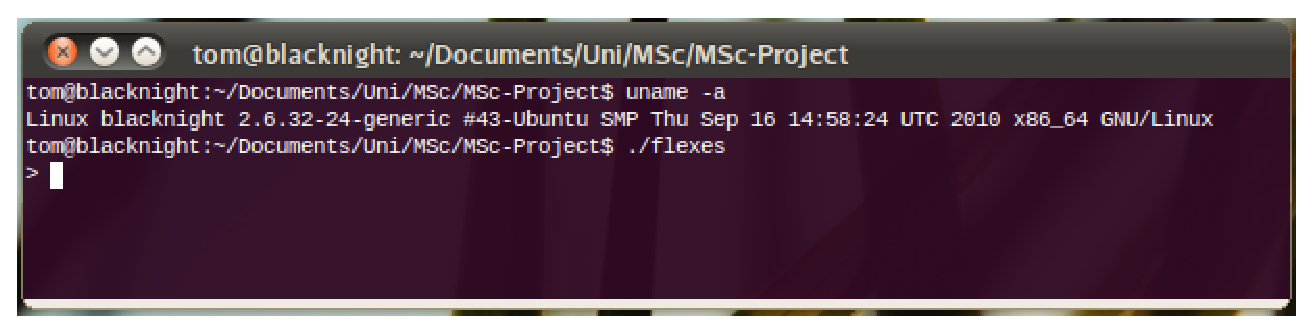
\includegraphics[scale=0.75]{linux}
	\caption{Running Ubuntu Linux, along with the compiler in text mode}\label{fig:linux}
\end{figure}
The compiler can also take an argument in the form of a flex file:
\begin{figure}[H]
	\centering
	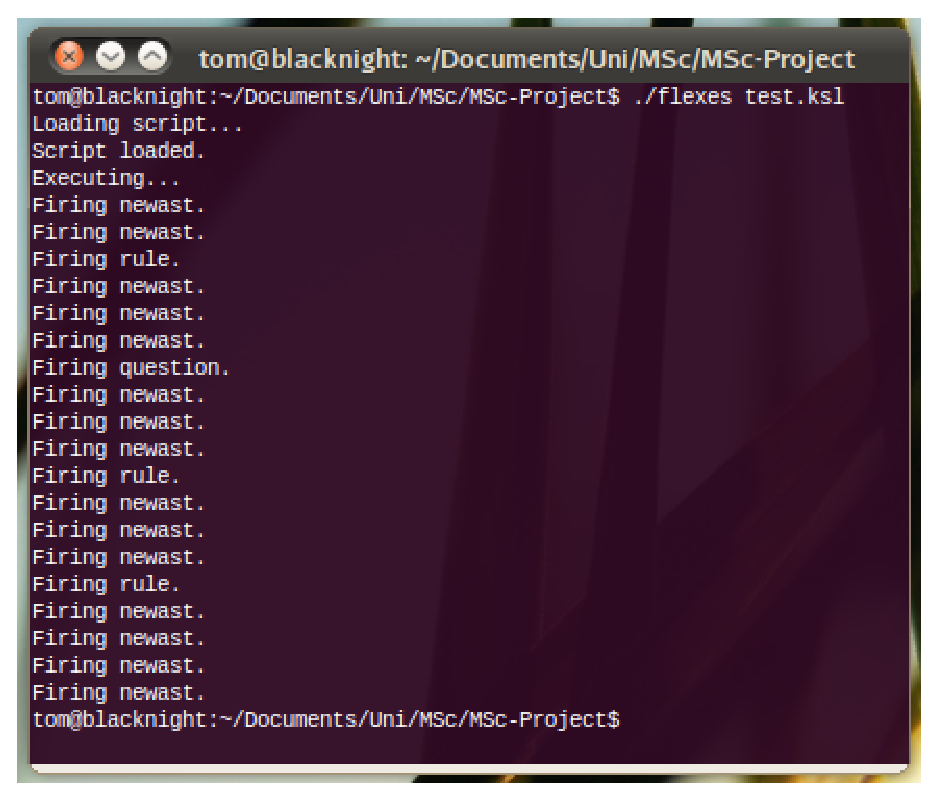
\includegraphics[scale=0.75]{flexes}
	\caption{The compiler (flexes) running a test script, without output.}\label{fig:flexes}
\end{figure}
In figure \ref{fig:flexes}, the compiler is reading from a source file that has been passed as an argument.\\
\\
Because the compiler is simple a source program without a graphical user interface, it doesn't make use of any library from Gnome or KDE.  If one wanted, a client could be built using GTK (Gnome) or QT (KDE) that would hook onto the flexes compiler.
\\
\\
Finally, the project is available on the github service.\\This can be found here: http://github.com/blackn1ght/MSc-Project.git
\section{What could have been done better?}\label{sec:con:better}
In hindsight, the project could have gone further based on a greater amount of research at the start.  Whilst there is a lot of material on creating a compiler, many of them go deep into the theoretical side, rather than anything practical that can be put into use, and then learn from that.\\
\\
The research into building compilers continuously provided answers to LLVM, the Low Level Virtual Machine discussed in section \ref{subsec:intermediate_code_gen}.  The switch from the C based code to C++ took some getting used to, and also attempting to hook into the LLVM functions.  Whilst using LLVM seemed like a good idea at the time, the lack of clear documentation or any practical examples seriously hindered development, and took a good chunk of time out of the development phase.\\
If the project were to be repeated with a greater amount of time, research into LLVM would need to be carried out first, however, it does seem a powerful 
\\
\\
Whilst AST's were put into place in the development, they weren't used in order to allow for a compliation.  A challenge was to get the variables to be used and declared at the same time, otherwise the compiler would complain that it could not find the symbol.  If there had been more time, more research could have been carried out in how to properly build the AST's, and generate a working WinFlex program.


\bibliographystyle{plainnat}
\bibliography{MSc-Dissertation}
\clearpage
\appendix
\appendixpage
\addappheadtotoc
Insert code dumpage here, or maybe not.. who knows?
\end{document}



